\documentclass[lang=en,mode=normal,device=normal,color=blue,12pt]{elegantnote}

\usepackage{amsmath,amssymb}
\usepackage{bbm}
\usepackage{tcolorbox}
\usepackage{graphicx}
\usepackage{booktabs}
\usepackage{subfig}
\usepackage{algorithm}
\usepackage{algpseudocode}
\usepackage[toc,page,title]{appendix}
\usepackage{hyperref}
\usepackage{float}

\setlength{\parindent}{0pt}


\DeclareMathOperator*{\1}{\mathbbm{1}}
\DeclareMathOperator*{\E}{\mathbb{E}}
\DeclareMathOperator*{\D}{\mathcal{D}}
\DeclareMathOperator*{\R}{\mathbbm{R}}
\DeclareMathOperator*{\argmax}{arg\,max}
\DeclareMathOperator*{\argmin}{arg\,min}

\title{Study Note: Reinforcement Learning Algorithms}

\author{Yanqing Wu\\[0.5cm]{Advisor: Prof. Hengshuai Yao}}
\institute{Viwistar Robotics}

\begin{document}
\maketitle

\tableofcontents

\newpage

\textit{Since some parts are not addressed directly from the literature, the explanations in this note are the best of my understanding.}

\newpage
\section{Taxonomy of reinforcement learning algorithms}

Reinforcement learning (RL) algorithms can be classified from different perspectives, including model-based and model-free methods, value-based and policy-based methods (or combination of the two), Monte Carlo methods and temporal-difference methods, on-policy and off-policy methods. Figure \ref{fig:taxonomy} provides an overview of RL algorithms.

\begin{figure}[!ht]
  \centering
  \makebox[\textwidth][c]{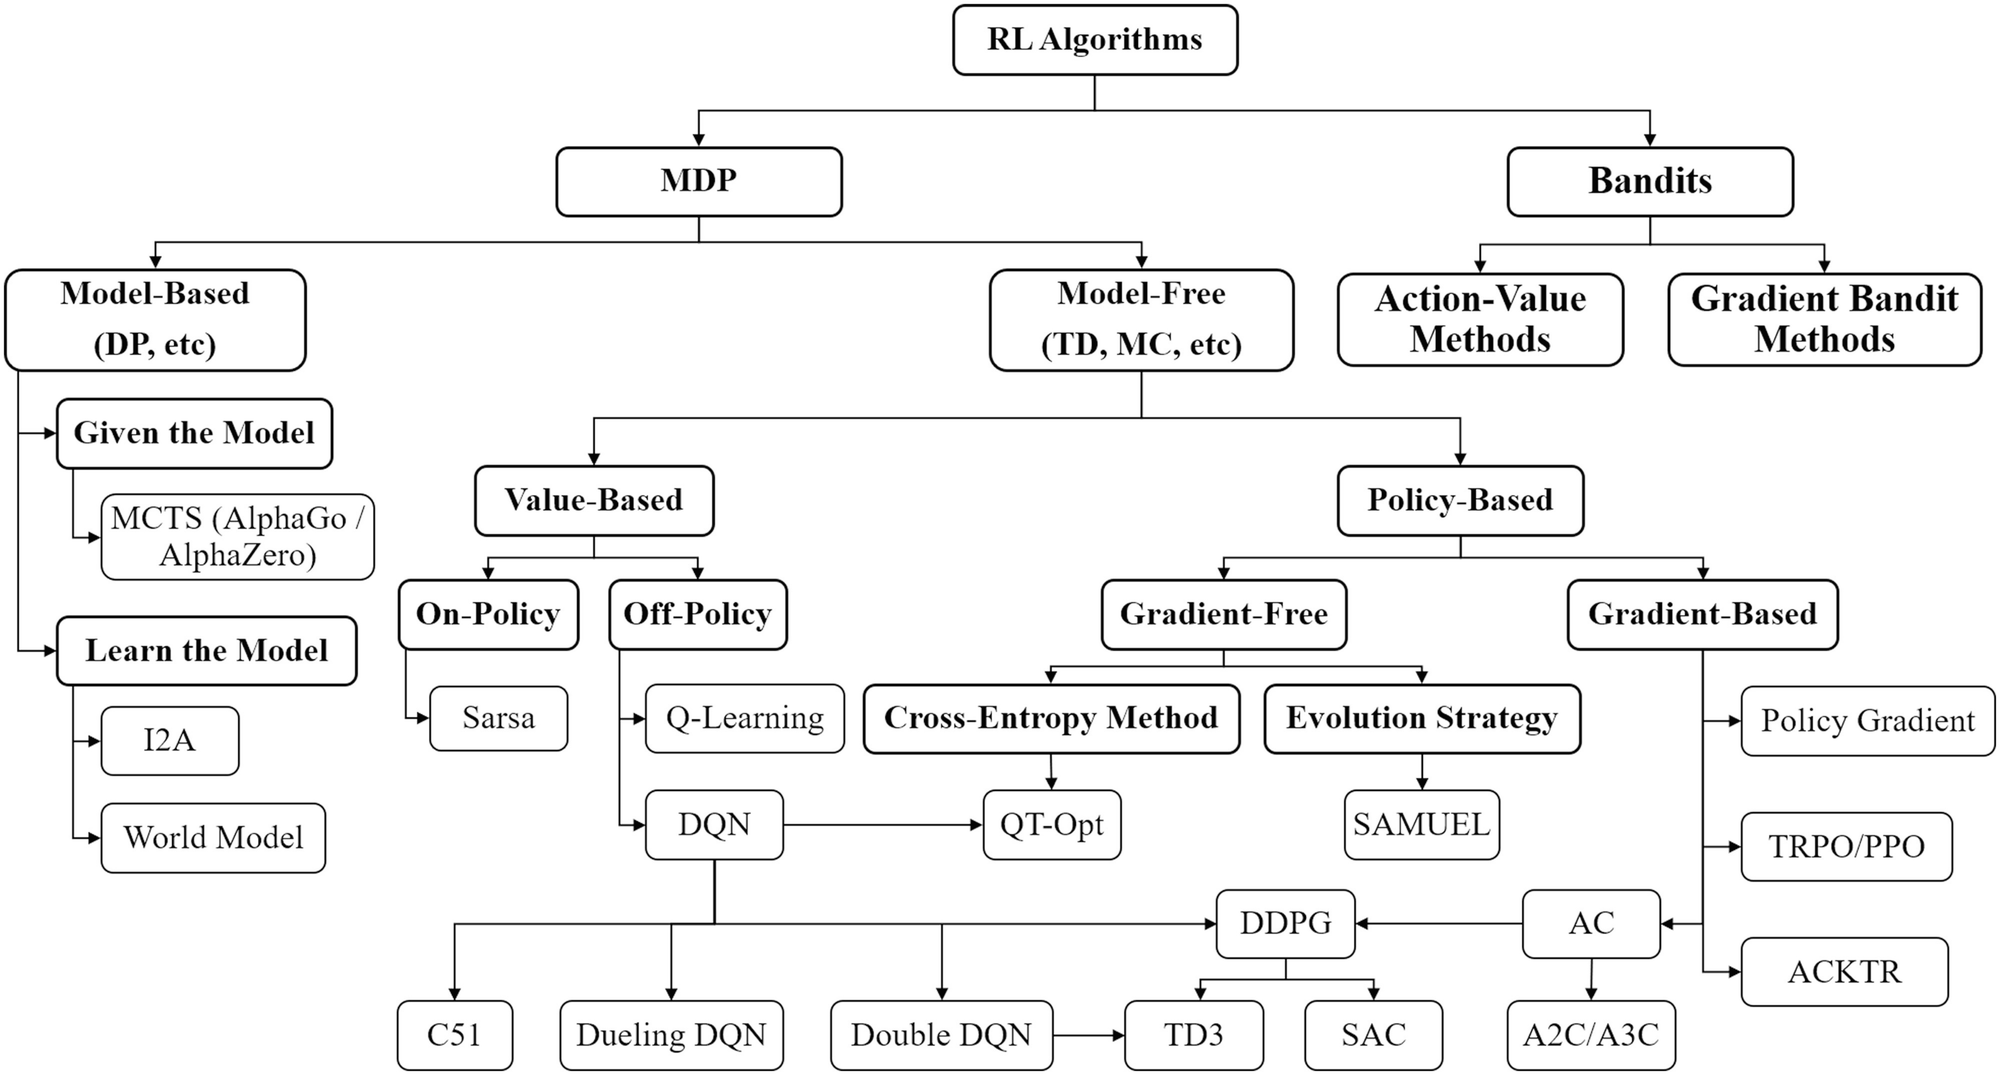
\includegraphics[width=1.2\linewidth]{taxonomy_rl.png}}%
  \caption{Map of RL algorithms. Boxes with thick lines denote different categories, others denote specific algorithms \cite{Zhang2020}}
  \label{fig:taxonomy}
\end{figure}

\subsection{Model-free vs. Model-based}
\label{appendix:model-dep}

You may have seen `model' referring to neural networks like in supervised learning.
In RL, the term `model' in `model-free' or `model-based' does NOT refer to neural networks or other statistical learning models.
To avoid ambiguity, neural networks are referred as `function approximators' in RL, which are often employed to learn and generalize value functions (such as Q values that predicts total return given a state-action pair).

Model-based RL has an agent try to understand the environment and create a `model' represent it.
\textbf{The transition function (probability distribution) from states $T$ and the reward function $R$ are called the `model' of the environment} (or Markov decision process, MDP).
From this model, the agent has a reference and can \textit{plan} accordingly. Model-free agent does not learn a model but instead learn a policy directly.

A RL agent is not `model-based' even there is a model of the environment implemented. A RL agent have to explicitly reference the `model' to be `model-based':

\begin{itemize}
\item `model-free' algorithms: algorithms that purely sample from experience (e.g. Monte Carlo control, SARSA, Q-learning, Actor-Critic)
\begin{itemize}
\item They rely on real samples from the environment and never use generated predictions of next state and next reward to alter behaviour. They might sample from experience memory (e.g. replay buffer), which is close to being a model.
\end{itemize}
\item archetypical `model-based' algorithms: Dynamic Programming (e.g. Policy Iteration, Value Iteration)
\begin{itemize}
\item They use the model's predictions or distributions of enxt state and reward to calculate optimal actions. In DP specifically, the model must provide state transition probabilities, and expected reward from any state, action pair.
\end{itemize}
\item other `model-based' algorithms: basic TD learning that only uses state values
\begin{itemize}
\item To pick the optimal action, it needs to ask a model that predicts what will happen on each action and implement a policy like $\pi(s) = argmax_a \sum_{s',r} p(s',r|s,a)(r+v(s'))$ where probability function $p(s',r|s,a)$ is essentially the model.
\end{itemize}
\end{itemize}

In short, model-based RL algorithms use models and planning to solve RL problems; model-free methods are explicitly trial-and-error learners (almost the opposite of planning).

A simple check to see if an RL algorithm is model-based or model-free is: \textit{if, after learning, the agent can make predictions about what the next state and reward will be before it takes each action, it is a model-based RL algorithm. If it cannot, then it is a model-free algorithm}.

% roll-out: The standard use of “rollout” (also called a “playout”) is in regard to an execution of a policy from the current state when there is some uncertainty about the next state or outcome - it is one simulation from your current state. 


\subsection{On-policy vs. Off-policy}
\label{appendix:on-off-policy}

By Prof. Yao, the key difference between the two is whether we use generated action to interact with the environment.

\begin{itemize}
\item On-policy learning: the same policy that is evaluated and improved is \textit{also} used to select actions.
\item Off-policy learning: the policy that is evaluated and improved (called estimation policy) is different from the policy that is used to select actions (called behaviour policy).
\end{itemize}

The on-policy methods, like SARSA, expects that the actions in every state are chosen based on the current policy of the agent, that usually tends to exploit rewards. By doing so, the policy gets better when we update our policy based on the last rewards. But, if we update our policy based on stored transitions, like in experience replay, we are actually evaluating actions from a policy that is no longer the current one.

An advantage of this separation is that the estimation policy may be deterministic (e.g. greedy), while the behaviour policy can continue to sample all possible actions.
Hence, off-policy gives us better exploration and helps us use data samples more efficiently.

Within off-policy methods, there are two types: Q learning and Q-based policy gradient (or Q-based actor critic) \cite{ytbcs287}.

\subsection{Policy-based vs. Value-based}

\begin{itemize}
\item policy-based: we explicitly build a representation of a policy (mapping $\pi:s\rightarrow a$) and keep it in memory during learning
\item value-based: we don't store any explicit policy, only a value function. The policy is here implicit and can be derived directly from the value function (pick the action with the best value)
\item actor-critic: a mix of policy-based (actor) and value-based (critic).
\end{itemize}

\subsubsection{Q-learning vs. Policy Gradient}

A more specific and symbolic example of policy-based vs value-based methods is: Q-learning (value-balsed) and Policy Gradient (policy-based).

In a post by \cite{qlearningvspg}: Both methods are theoretically driven by the Markov Decision Process construct, and as a result use similar notation and concepts. In addition, in simple solvable environments you should expect both methods to result in the same, or at least equivalent, optimal policies.

However, they are actually different internally. The most fundamental differences between the approaches is in how they approach action selection, both whilst learning, and as the output (the learned policy). In Q-learning, the goal is to learn a single deterministic action from a discrete set of actions by finding the maximum value. With policy gradients, and other direct policy searches, the goal is to learn a map from state to action, which can be stochastic, and works in continuous action spaces.

As a result, policy gradient methods can solve problems that value-based methods cannot:
\begin{itemize}
\item Large and continuous action space. However, with value-based methods, this can still be approximated with discretisation - and this is not a bad choice, since the mapping function in policy gradient has to be some kind of approximator in practice.
\item Stochastic policies. A value-based method cannot solve an environment where the optimal policy is stochastic requiring specific probabilities, such as Scissor/Paper/Stone. That is because there are no trainable parameters in Q-learning that control probabilities of action, the problem formulation in TD learning assumes that a deterministic agent can be optimal.
\end{itemize}
However, value-based methods like Q-learning have some advantages too:
\begin{itemize}
\item Simplicity. You can implement Q functions as simple discrete tables, and this gives some guarantees of convergence. There are no tabular versions of policy gradient, because you need a mapping function $p(a|s,\theta)$ which also must have a smooth gradient with respect to $\theta$.
\item Speed. TD learning methods that bootstrap are often much faster to learn a policy than methods which must purely sample from the environment in order to evaluate progress.
\end{itemize}
There are other reasons why you might care to use one or other approach:
\begin{itemize}
\item You may want to know the predicted return whilst the process is running, to help other planning processes associated with the agent.
\item The state representation of the problem lends itself more easily to either a value function or a policy function. A value function may turn out to have very simple relationship to the state and the policy function very complex and hard to learn, or vice-versa.
\end{itemize}

Some state-of-the-art RL solvers actually use both approaches together, such as Actor-Critic. This combines strengths of value and policy gradient methods.

\newpage

\section{Algorithms}

\subsection{PPO}

\subsubsection{Introduction}

In normal policy gradient, training can be unstable due to sparse reward and sampled target, causing dramatic changes on the policy; this eventually collapses performance.
To enhance training stability, we want to limit the parameter updates that would change the policy too much at one step\footnote{In supervised learning, it will be corrected on the next update. In RL, step too far results in terrible policy and new data will be collected in this policy, therefore cannot be self-corrected.}.
With this goal, True Region Policy Optimization (TRPO) \cite{schulman2017trust} was introduced.
TRPO delimit the KL-divergence with a constraint. More specifically, TRPO updates policies by taking the largest step possible to improve performance while satisfying the constraint on how close the new and old policies are allowed to be \footnote{Trust Region is a more advanced \textit{step-sizing} method than line search along gradient}.
However, TRPO is complicated to implement and is computational-heavy (from the computation of second-order derivatives of KL-divergence). Proximal Policy Optimization (PPO) \cite{schulman2017proximal} simplifies it by using a \textit{clipped surrogate objective} while retaining similar constraints and similar performance.
Instead of enforcing a hard constraint as in TRPO, PPO formalized the constraint as a penalty in the objective function.

There are two primary variants of PPO: PPO-Clip and PPO-Penalty.
\newline
\textbf{PPO-Clip} does not have a KL-divergence term in the objective and does not have a constraint at all. Instead relies on specialized clipping in the objective function to remove incentives for the new policy to drift from the old policy, PPO does hard clipping the policy ratio to be within a small range around 1.0, where 1.0 means the new policy is the same as old.
\newline
\textbf{PPO-Penalty} approximately solves a KL-constrained update like TRPO, but penalizes the KL-divergence in the objective function instead of making it a hard constraint, and automatically adjusts the penalty coefficient throughout training so that it is scaled appropriately.
PPO-Penalty performs worse than PPO-Clip \cite{schulman2017proximal}.

% PPO combines ideas from A2C (having multiple workers) and TRPO (it uses a trust region to improve the actor).
%The main idea is that after an update, the new policy should be not too far from the old policy. For that, PPO uses clipping to avoid too large updates.






\subsubsection{Implementation}


% https://towardsdatascience.com/proximal-policy-optimization-tutorial-part-1-actor-critic-method-d53f9afffbf6
% https://towardsdatascience.com/proximal-policy-optimization-tutorial-part-2-2-gae-and-ppo-loss-fe1b3c5549e8
PPO uses the Actor-Critic approach. It uses two models, Actor Model and Critic Model, as shown in Figure \ref{fig:ppo_ac}.

% TODO: use tikz
\begin{figure}[!ht]
  \centering
  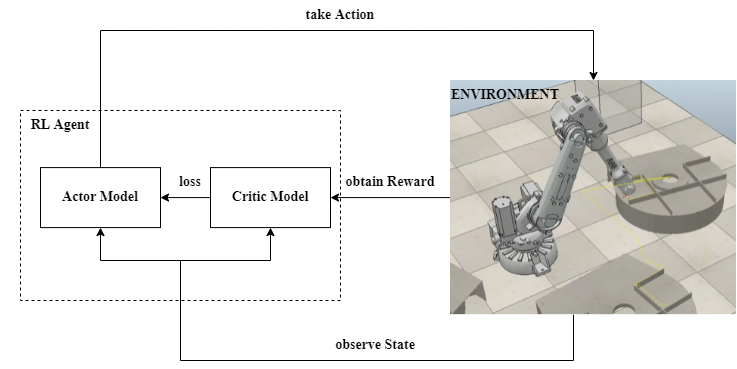
\includegraphics[width=0.9\linewidth]{PPO_AC.PNG}
  \caption{PPO agent}
  \label{fig:ppo_ac}
\end{figure}

The Actor model (policy $\pi$) learns what action to take under a particular observed state of the environment.
% In our case, it may take joint angles, obstacle positions and/or collisions as inputs and gives tip pose as action for output. 
The action predicted by the actor is sent to the environment. Afterwards, observation is made and reward is given from the environment and fed into the Critic Model.

The Critic model (value $V(s)$) learns to evaluate changes in the environment after action is taken by the Actor, and gives its feedback to the Actor. It outputs a real number indicating a rating (Q-value) of the action taken in the previous state. By comparing this rating obtained from the Critic, the Actor compares its current policy with a new policy and decides how it wants to improve itself to take better actions.



\paragraph{OpenAI PPO}
The pseudocode of PPO algorithm is shown in Figure \ref{fig:ppo}.
\begin{figure}[h!]
  \centering
  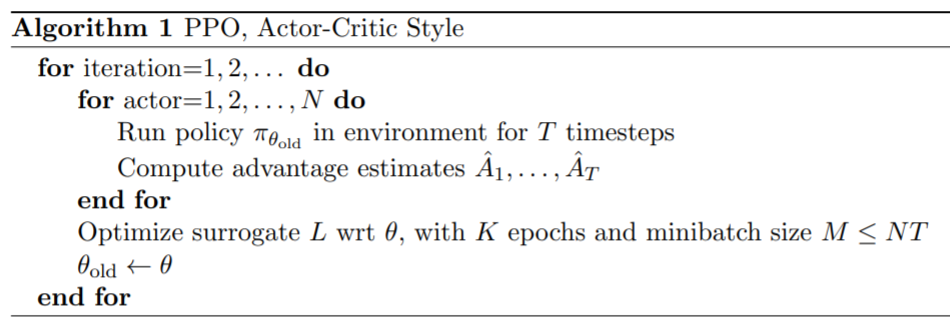
\includegraphics[width=0.7\linewidth]{ppo_openai.PNG}
  \caption{Screenshot of OpenAI PPO algorithm}
  \label{fig:ppo}
\end{figure}

\subparagraph{Key components}

Policy loss, value function loss, KL loss (optional) and entropy regularization make up the loss for PPO.

\textit{Probability Ratio} $r_t(\theta)$ calculates how much the policy has changed. This ratio decides the tolerance of a change in policy. A clipping parameter epsilon $\epsilon$ is used to ensure only the maximum of $\epsilon$ change is made to the policy at a time. $r_t(\theta) > 1$ means the action is more probable for the current policy than the old policy.
\[
r_t(\theta) = \frac{\pi_{\theta} (a_t | s_t)}{\pi_{\theta_\text{old}} (a_t | s_t)} = \frac{\pi_{new}(\theta)}{\pi_{old}(\theta)} \overset{\mathrm{\text{computational convenience}}}= e^{ log(\pi_{new}(\theta)) - log(\pi_{old}(\theta)) }
\]


% https://stackoverflow.com/questions/46422845/what-is-the-way-to-understand-proximal-policy-optimization-algorithm-in-rl
% A-hat could be the discounted return (as in REINFORCE) or the advantage function (as in GAE) for example
\textit{Advantage} $\hat{A}$ measures how much better or worse by taking a particular action in a particular state. Advantage is computed using Generalized Advantage Estimator (GAE($\lambda$)). Truncated version of advantage estimator $\hat{A_t}$ is given by
\begin{align*}
\hat{A_t} & = \delta_t + (\gamma \lambda)\delta_{t+1} + \cdots + (\gamma\lambda)^{T-t+1}\delta_{T-1} \\
\delta_t & = r_t + \gamma V(s_{t+1}) - V(s_t)
\end{align*}

\textit{Actor Loss}, or \textit{Policy (Gradient) loss} $L^{CLIP}$ is defined as a minimum of two functions in PPO. The first function $p_1$ is a surrogate loss function from conservative policy iteration ($L^{CPI}$), which is from TRPO \cite{schulman2017trust}.
The second function $p_2$ is the clipped probability ratio, which $r_t(\theta)$ is limited within the interval $[1-\epsilon, 1+\epsilon]$ ($\epsilon$ is clipping range).
The minimum of the two is taken so that the final objective is a lower bound (i.e. a \textit{pessimistic bound}) on the unclipped objective.
\begin{align*}
p_1 & = \text{ratio}\cdot\text{advantage} = r_t(\theta)\cdot\hat{A_t}\\
p_2 & = \text{clip}(\text{ratio}, 1-\epsilon, 1+\epsilon)\cdot\text{advantage} = clip(r_t(\theta), 1-\epsilon, 1+\epsilon)\cdot\hat{A_t}\\
L^{CLIP}(\theta) & = min(p_1, p_2) = \hat{\E_t}[min(r_t(\theta)\hat{A_t},clip(r_t(\theta),1-\epsilon,1+\epsilon)\hat{A_t})]
\end{align*}

Based on my understanding from \cite{ppocs294}, to illustrate why the minimum of the two functions is chosen, see Figure \ref{fig:mm_algo} below.
\begin{figure}[!ht]
  \centering
  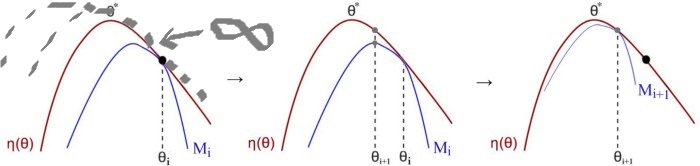
\includegraphics[width=0.9\linewidth]{MM_lowerbound.jpeg}
  \caption{Minorize-Maximization (MM) Algorithm}
  \label{fig:mm_algo}
\end{figure}
Think of the red line as a true objective function, and the blue line as a local approximation.
If we choose to maximize all the way, the approximation will go to infinity.
If we take local approximation and subtract a penalty, we receive a lower bound on the true objective function.
When we make progress on this pessimistic version of the objective, we are guaranteed to make progress and eventually converge on the true objective function . The idea behind this is Minorize-Maximization Algorithm.
Alternatively by \cite{weng2018PG}, the minimum is chosen because we avoid increasing the policy update to extremes for better rewards.

Policy loss correlates to how much the policy (process for deciding actions) is changing.
The magnitude of this should decrease during a successful training session.
These values will oscillate during training. Generally they should be less than 1.0.


Another version of $L^{CLIP}$ is as follows:
$$ L(s,a,\theta_k,\theta) = \min\left(
\frac{\pi_{\theta}(a|s)}{\pi_{\theta_k}(a|s)}  A^{\pi_{\theta_k}}(s,a), \;\;
g(\epsilon, A^{\pi_{\theta_k}}(s,a))
\right) $$
where $g(\epsilon,A) = (1+\epsilon)A$ when $A \geq 0$ and $g(\epsilon,A) = (1-\epsilon)A$ when $A < 0$. Through some simplifications, we see that probability ratio $\frac{\pi_{\theta}(a|s)}{\pi_{\theta_k}(a|s)}$ is clipped at $1+\epsilon\;(A>0)$ and $1-\epsilon\;(A<0)$. The hyperparameter $\epsilon$ specifies how much the new policy is allowed to change from the old policy (while still profiting the objective). Therefore, the clipping acts as a regularizer by discouraging the policy to change dramatically (see Figure \ref{fig:lclip}).

\begin{figure}[!ht]
  \centering
  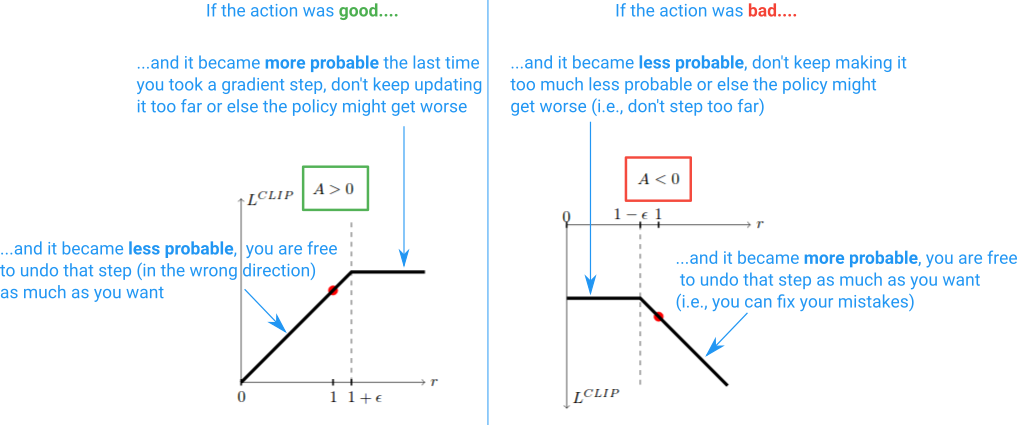
\includegraphics[width=0.9\linewidth]{LCLIP.PNG}
  \caption{Effect of $L^{CLIP}$ function \cite{ppolclip}}
  \label{fig:lclip}
\end{figure}

\textit{Critic Loss}, or \textit{Value (Function) Loss} $L^{VF}$ is defined as mean squared error between critic values and returns (or $V_t^{target}$ in the paper).
Target value is computed using TD($\lambda$) estimator.
Value Loss correlates to how well the model is able to predict the value of each state.
This should increase while the agent is learning, and then decrease once the reward stabilizes.
These values will increase as the reward increases, and then should decrease once reward becomes stable.
\[
L^{VF} = (V(s) - R)^2 = (V_\theta(s_t) - V_t^{target})^2
\]

\textit{Total Loss}, or \textit{Objective Loss} $L_t^{CLIP+VF+S}$ is defined as\footnote{The plus/minus sign of each loss component differs from source to source. The sign of the first (text) equation is align with PPO2 source code and some online post; the sign of the second (letter) equation is align with the paper.}\footnote{Based on discussion with the Advisor, the plus/minus sign of the first (text) equation should be the correct version. We must maximize entropy to minimize loss, hence the minus sign before entropy.}:
\begin{align*}
\text{total loss} & = \text{actor loss} + \text{critic loss} - \text{entropy} \\
L_t^{CLIP+VF+S}(\theta) & = \hat{\E_t} [L_t^{CLIP}(\theta) - c_1 L_t^{VF} + c_2 S[\pi_\theta](s_t)]
\end{align*}
where $c_1, c_2$ are coefficients, $\theta$ is a vector of policy parameters, $S$ is entropy bonus that acts as a regularizer to encourage policy exploration (see Appendix \ref{appendix:entropy} for more information of \textit{Entropy}).

Note that actor loss ($L_t^{CLIP}$) and critic loss ($L_t^{VF}$) correspond to exploitation, and entropy regularization ($S$) corresponds to exploration. The total loss equation here is a trade-off problem between exploitation and exploration, which is one of the key features and challenges in RL problems.


\subparagraph{Practical considerations}

There are two alternating threads in PPO. In the first thread, policy interacts with the environment, collects data and computes advantage estimates (using fitted baselines estimates); in the second thread, it collects all the experiences and runs Stochastic Gradient Descent (SGD) to optimize the policy using the clipped objective.

The surrogate loss $L$ is optimized with minibatch SGD on $NT$ timesteps of data, where $N$ is the number of parallel actors and $T$ is timesteps.



\paragraph{DeepMind PPO}

DeepMind paper provides a more detailed pseudocode than OpenAI. According to DeepMind pseudo-code of PPO (\ref{fig:ppo})

\begin{figure}[h!]
  \centering
  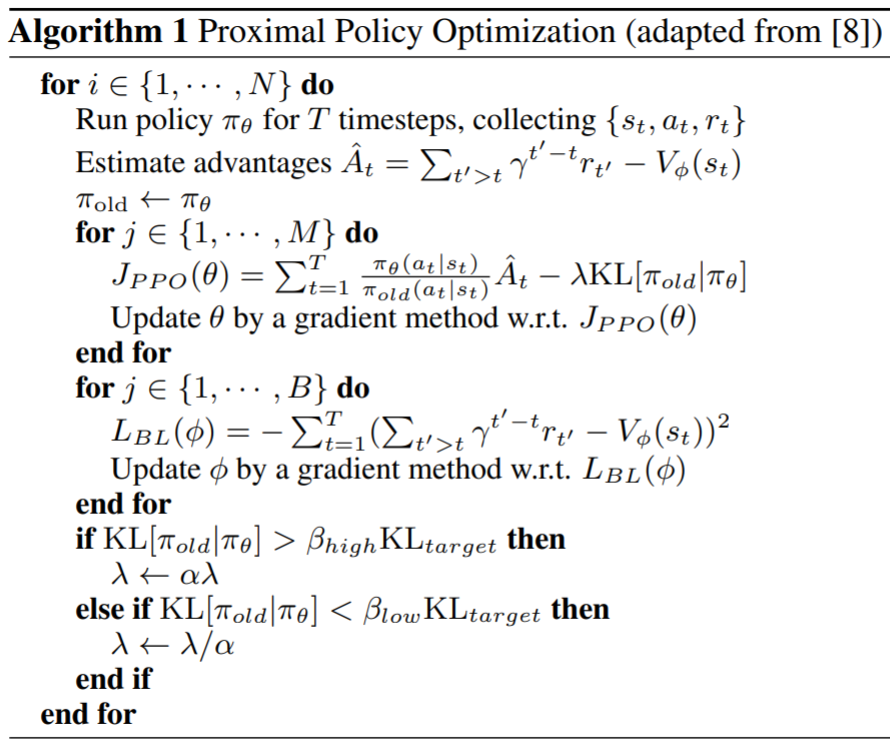
\includegraphics[width=0.7\linewidth]{ppo.PNG}
  \caption{Screenshot of DeepMind PPO algorithm}
  \label{fig:ppo}
\end{figure}

In this algorithm, $KL_{target}$ is the desired change in the policy per iteration.
The Actor maximizes $J_{PPO}$, and Critic minimizes $L_{BL}$.

\subsubsection{PPO1 vs. PPO2}

PPO2 is made for GPU by OpenAI. It uses vectorized environments for multi-processing while PPO1 uses MPI. PPO2 contains several modifications from the original algorithm which are not documented by OpenAI: value function is also clipped and advantages are normalized \cite{ppo2stable}.

PPO1 is not gpu-optimized: it uses one environment per MPI worker. In other words, when running PPO1 with multiple MPI processes, each process creates its own copy of the environment, and its own neural net (NN). The gradients for NN updates are aggregated across the workers by virtue of using MpiAdamOptimizer class.
PPO2 implementation (while with recent updates it can use MPI as well) uses a different version of parallelism. Head process with a single neural net creates a bunch of subprocesses that run separate environments (run environments means that take actions and produce next observations and rewards).
The observations and rewards from these multiple environments in subprocesses are batched together in the head process.
For visual observations, that creates a big enough batch so that computation of NN gradients on a GPU starts making sense.
By default, multiple environments in subprocesses are only used for atari and retro video games, but not, for instance, for mujoco (because observations there are not visual) \cite{ppo2vsppo1}.

In conclusion, PPO1 is obsolete at the time of writing this note, and its functionality is fully covered by PPO2.


\paragraph{OpenAI source code of PPO}

\begin{itemize}
\item PPO1: \url{https://github.com/openai/baselines/blob/master/baselines/ppo1/pposgd_simple.py}
\item PPO2: \url{https://github.com/openai/baselines/blob/master/baselines/ppo2/model.py}
\end{itemize}

\subsubsection{Improvement}

In a later paper by \cite{hsu2020revisiting}, two common design choices in PPO are revisited, precisely (1) clipped probability ratio for policy regularization and (2) parameterize policy action space by continuous Gaussian or discrete softmax distribution. They first identified three failure modes in PPO and proposed replacements for these two designs.

The failure modes are:
\begin{itemize}
\item On continuous action spaces, standard PPO is unstable when rewards vanish outside bounded support.
\item On discrete action spaces with sparse high rewards, standard PPO often gets stuck at suboptimal actions.
\item The policy is sensitive to initialization when there are locally optimal actions close to initialization.
\end{itemize}


Discretizing the action space or use Beta distribution helps avoid failure mode 1\&3 associated with Gaussian policy. Using KL regularization (same motivation as in TRPO) as an alternative surrogate model helps resolve failure mode 1\&2.



\newpage
\subsection{SAC}

\subsubsection{Introduction}



Model-free deep reinforcement learning (RL) algorithms are proven to work on decision making and control tasks. However, these methods are hindered by two major challenges: very high sample complexity (requires at least millions of steps of data collection) and brittle convergence properties (extremely sensitive to hyperparameters).
One cause for the high sample complexity (or poor sample efficiency) is on-policy learning. On-policy learning methods, such as TRPO, PPO, or A3C, require collecting new samples for each gradient step and which is extremely expensive.
To improve sample efficiency, we need to reuse past experience (or `experience replay' in literature), which requires off-policy algorithms  \cite{mnih2013playing}. However, off-policy variants based on soft Q-learning require complex approximate inference procedures in continuous action spaces. 
% https://web.stanford.edu/class/psych209/Readings/MnihEtAlHassibis15NatureControlDeepRL.pdf


Soft Actor Critic \cite{haarnoja2018soft}, or SAC, was introduced to provide both sample efficiency and stability in continuous action spaces, and extendability to complex and high-dimensional tasks. SAC is an off-policy actor-critic deep RL algorithm based on the maximum entropy framework. In this framework, the actor aims to maximize expected reward as well as entropy. That is, to succeed at the task while acting as randomly as possible. Prior deep RL methods based on this framework have been formulated as Q-learning methods. SAC combines off-policy updates with a stable stochastic actor-critic formulation.


%\url{https://spinningup.openai.com/en/latest/algorithms/sac.html}
%
%\url{https://towardsdatascience.com/soft-actor-critic-demystified-b8427df61665}
%
%\url{https://spinningup.openai.com/en/latest/spinningup/rl_intro.html}

\subsubsection{Implementation}

Three key components in SAC:

\begin{itemize}
\item An actor-critic architecture with separate policy and value function networks;
\item An off-policy formulation that enables reuse of previously collected data for efficiency;
\item Entropy maximization to enable stability and exploration.
\end{itemize}

The policy is trained with the \textit{objective} to maximize the expected return and the entropy at the same time:
\[
J(\theta) = \sum_{t=1}^T \E_{(s_t, a_t) \sim \rho_{\pi_\theta}} [r(s_t, a_t) + \alpha \mathbb{H} (\pi_\theta(\cdot | s_t))]
\]
where $\mathbb{H}(\cdot)$ is the entropy measure and $\alpha$ (temperature parameter) controls how important the entropy term is.
The entropy maximization leads to policies that can (1) explore more and (2) capture multiple modes of near-optimal strategies (i.e., if there exist multiple options that seem to be equally good, the policy should assign each with an equal probability to be chosen).

Precisely, SAC aims to learn three functions:

\begin{itemize}
\item $\pi_\theta$, the policy with parameter $\theta$
\item $Q_w$, soft Q-value function parameterized by $w$
\item $V_\psi$, soft state-value function parameterized by $\psi$
\end{itemize}

\textit{Soft Q-value} (or soft action value) and \textit{soft state value} are defined as:
\begin{align*}
Q(s_t, a_t) &= r(s_t, a_t) + \gamma \mathbb{E}_{s_{t+1} \sim \rho_{\pi}(s)} [V(s_{t+1})] & \text{; according to Bellman equation.}\\
\text{where }V(s_t) &= \mathbb{E}_{a_t \sim \pi} [Q(s_t, a_t) - \underbrace{\alpha \log \pi(a_t | s_t)}_\text{entropy}] & \text{; soft state value function.}
\end{align*}
\[
\text{Thus, } Q(s_t, a_t) = r(s_t, a_t) + \gamma \mathbb{E}_{(s_{t+1}, a_{t+1}) \sim \rho_{\pi}} [Q(s_{t+1}, a_{t+1}) - \alpha \log \pi(a_{t+1} \vert s_{t+1})]
\]
$\rho_\pi (s_t)$ and $\rho_\pi(s_t, a_t)$ denote the state and state-action marginals of the trajectory (state) distribution included by a policy $\pi (a_t |s_t)$.

The \textit{soft state value function} is trained to minimize the mean square error:
\begin{align*}
J_V(\psi) &= \mathbb{E}_{s_t \sim \mathcal{D}} [\frac{1}{2} \big( \underbrace{V_\psi(s_t)}_\text{value} - \mathbb{E}[\underbrace{Q_w(s_t, a_t)}_\text{target} - \underbrace{\log \pi_\theta(a_t \vert s_t)}_\text{entropy}] \big)^2] \\
\text{with gradient: }\nabla_\psi J_V(\psi) &= \nabla_\psi V_\psi(s_t)\big( V_\psi(s_t) - Q_w(s_t, a_t) + \log \pi_\theta (a_t \vert s_t) \big)
\end{align*}
where $\mathcal{D}$ is the replay buffer.

The \textit{soft Q function} is trained to minimize the soft Bellman residual:
\begin{align*}
J_Q(w) &= \mathbb{E}_{(s_t, a_t) \sim \mathcal{D}} [\frac{1}{2}\big( Q_w(s_t, a_t) - \underbrace{(r(s_t, a_t) + \gamma \mathbb{E}_{s_{t+1} \sim \rho_\pi(s)}[V_{\bar{\psi}}(s_{t+1})])}_\text{target} \big)^2] \\
\text{with gradient: } \nabla_w J_Q(w) &= \nabla_w Q_w(s_t, a_t) \big( Q_w(s_t, a_t) - r(s_t, a_t) - \gamma V_{\bar{\psi}}(s_{t+1})\big)
\end{align*}
where $\bar{\psi}$ is the target value function which is the exponential moving average (or only gets updated periodically in a `hard' way), just like how the parameter of the target Q network is treated in DQN to stabilize the training.

SAC updates the policy to minimize the KL-divergence:
\begin{align*}
\pi_\text{new} 
&= \arg\min_{\pi' \in \Pi} D_\text{KL} \Big( \pi'(\cdot | s_t) \| \frac{\exp(Q^{\pi_\text{old}}(s_t, \cdot))}{Z^{\pi_\text{old}}(s_t)} \Big) \\[6pt]
&= \arg\min_{\pi' \in \Pi} D_\text{KL} \big( \pi'(\cdot | s_t) \| \exp(Q^{\pi_\text{old}}(s_t, \cdot) - \log Z^{\pi_\text{old}}(s_t)) \big) \\[6pt]
\text{objective for update: } J_\pi(\theta) &= \nabla_\theta D_\text{KL} \big( \pi_\theta(\cdot | s_t) \| \exp(Q_w(s_t, \cdot) - \log Z_w(s_t)) \big) \\[6pt]
&= \mathbb{E}_{a_t\sim\pi} \Big[ - \log \big( \frac{\exp(Q_w(s_t, a_t) - \log Z_w(s_t))}{\pi_\theta(a_t | s_t)} \big) \Big] \\[6pt]
&= \mathbb{E}_{a_t\sim\pi} [ \log \pi_\theta(a_t | s_t) - Q_w(s_t, a_t) + \log Z_w(s_t) ]
\end{align*}
where $\Pi$ is the set of potential policies that we can model our policy as to keep them tractable; e.g., $\Pi$ can be the family of Gaussian mixture distributions, expensive to model but highly expressive and still tractable.
$Z^{\pi_{\text{old}}}(s_t)$ is the partition function to normalize the distribution.
It is usually intractable but does not contribute to the gradient. How to minimize $J_\pi (\theta)$ depends our choice of $\Pi$.

This update guarantees that $Q^{\pi_\text{new}}(s_t, a_t) \geq Q^{\pi_\text{old}}(s_t, a_t)$, please check the proof on this lemma in the Appendix B.2 in \cite{haarnoja2018soft}.

Once we have defined the objective functions and gradients for soft action-state value, soft state value and the policy network, the soft actor-critic algorithm is as follows:
\begin{figure}[h!]
  \centering
  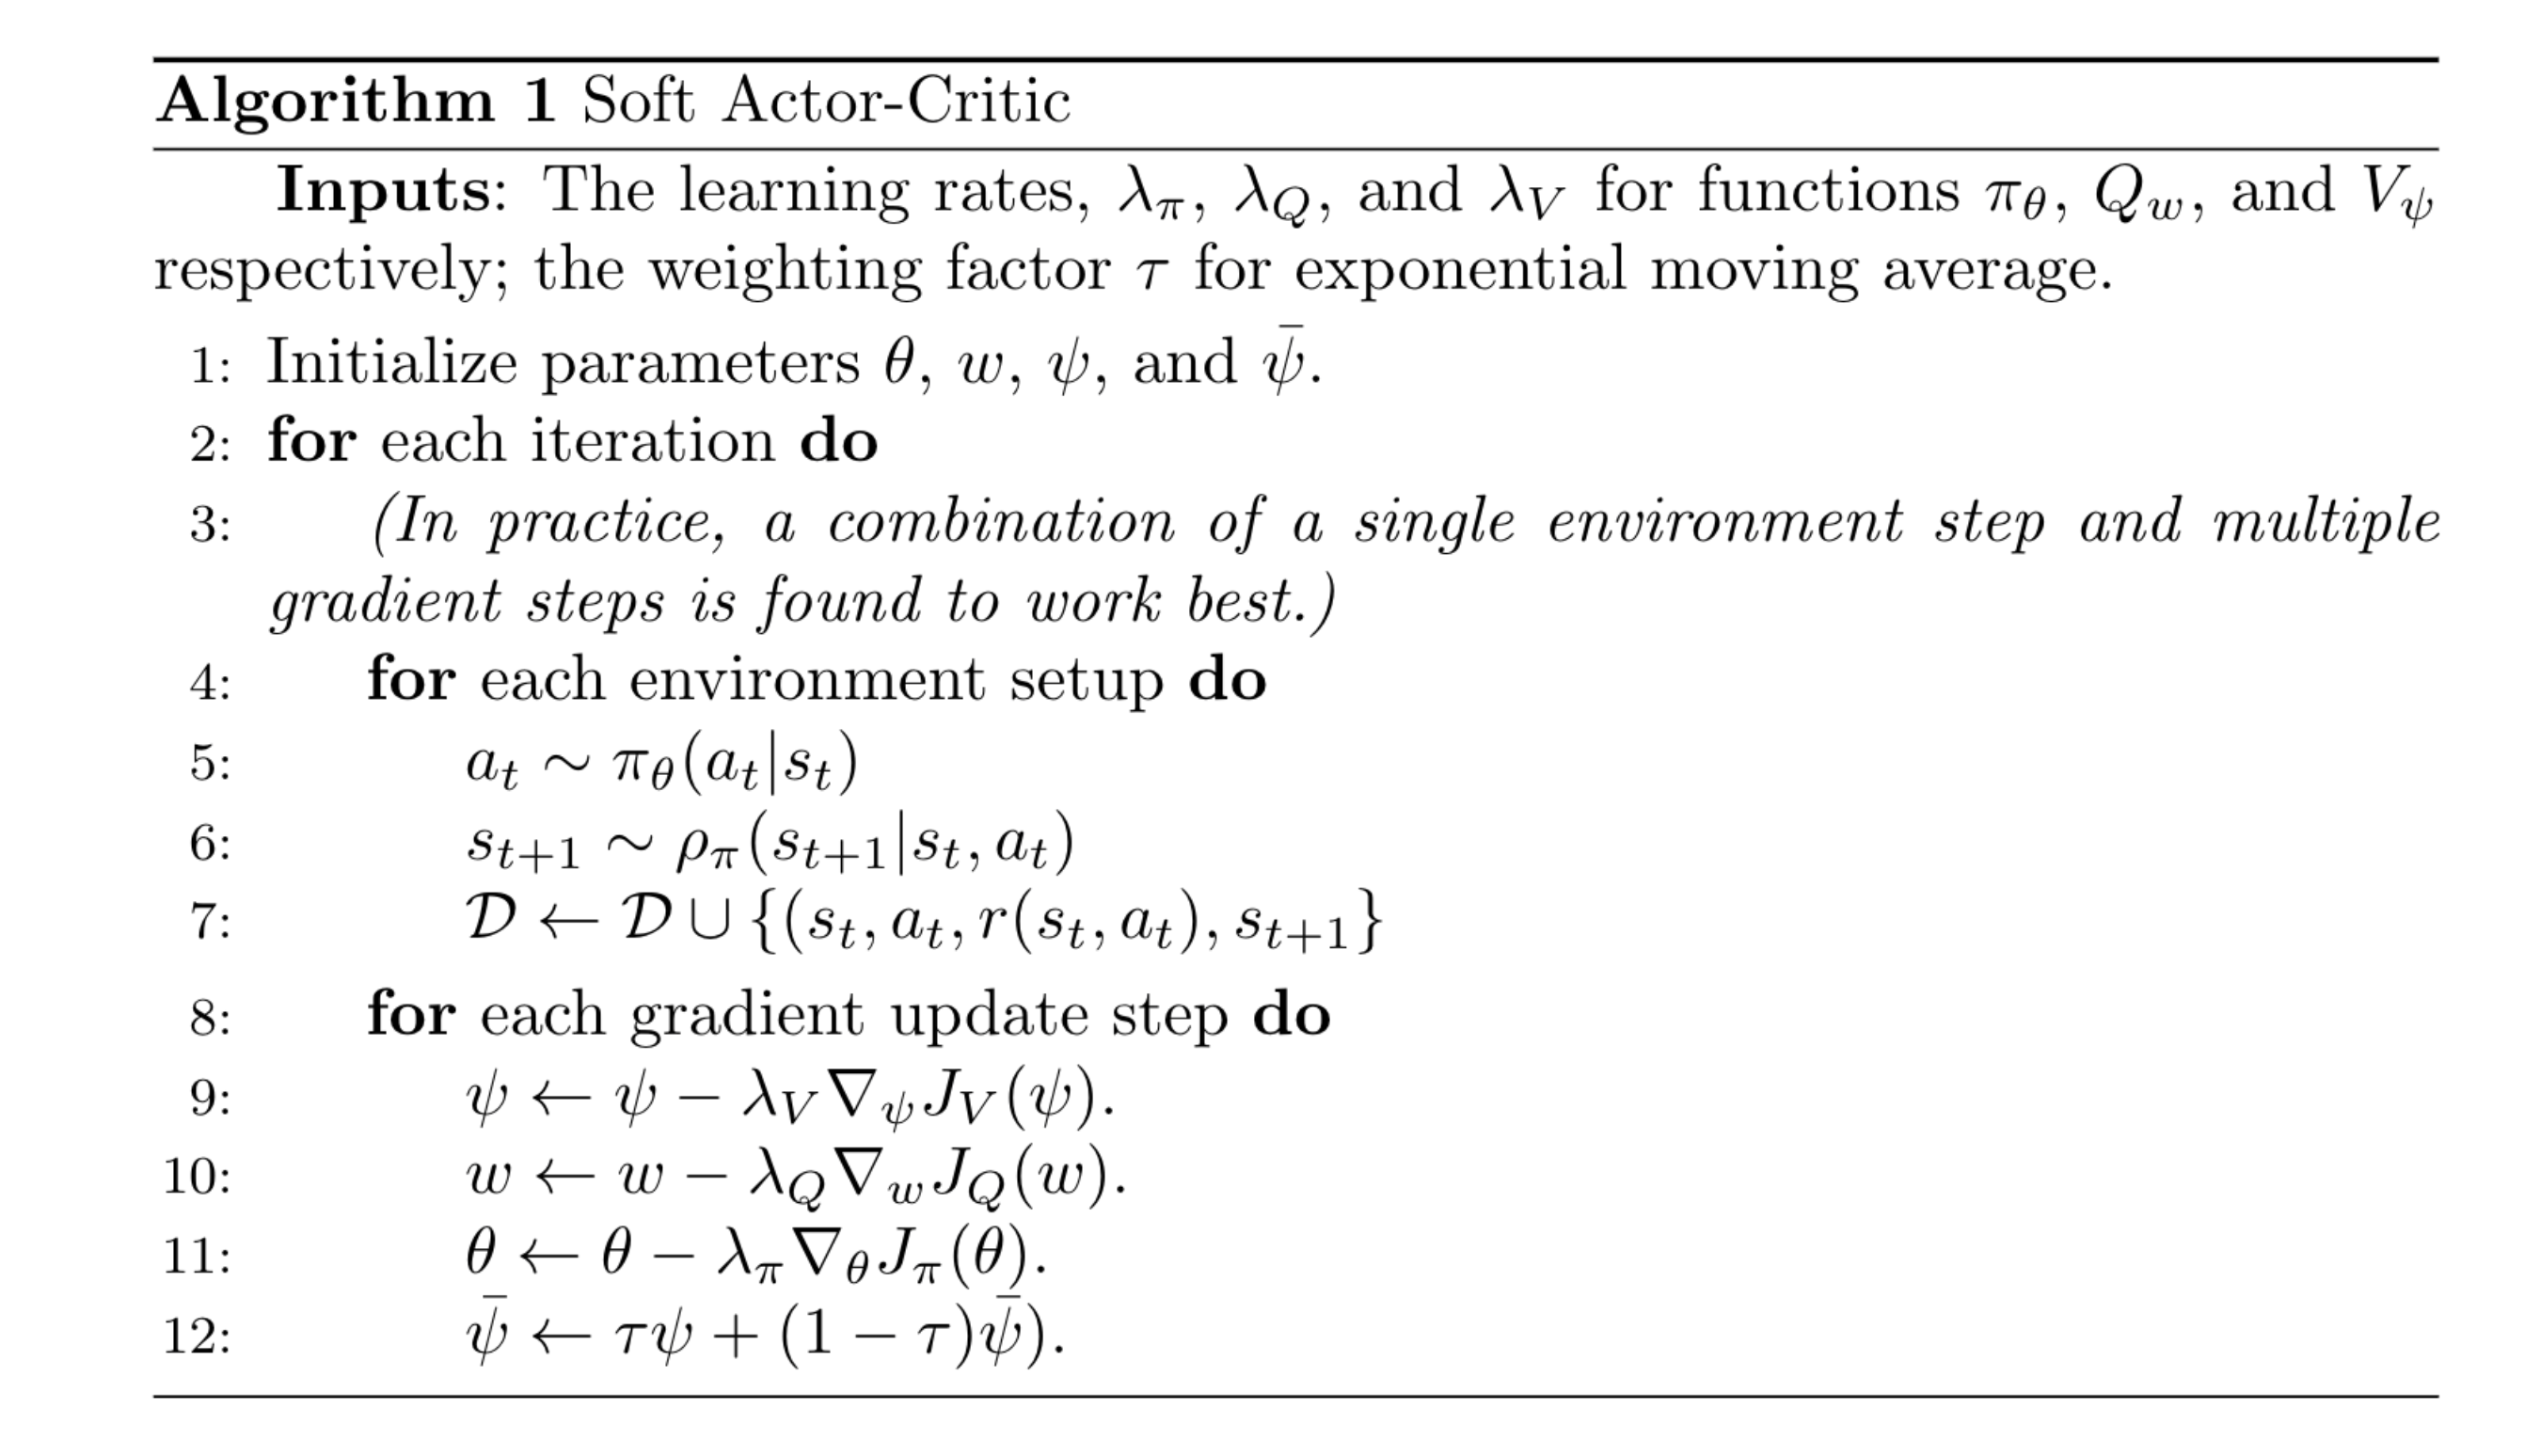
\includegraphics[width=0.9\linewidth]{SAC_algo.png}
  \caption{Screenshot of SAC algorithm}
  \label{fig:SAC_algo}
\end{figure}

\paragraph{Source Code}
\url{https://github.com/haarnoja/sac}

\subsubsection{Improvement}

\paragraph{SAC with automatically adjusted temperature}

SAC is brittle with respect to the temperature parameter.
Unfortunately it is difficult to adjust temperature, because the entropy can vary unpredictably both across tasks and during training as the policy becomes better.
An improvement on SAC formulates a constrained optimization problem: while maximizing the expected return, the policy should satisfy a minimum entropy constraint \cite{haarnoja2019soft}.


\subsubsection{Further reading}
%%%%%%%%%%%%%%%%%%%%%%%%%%
%%compute efficiency vs. sample efficiency, where SAC outperforms PPO in sample efficiency
%
\begin{itemize}
\item \href{https://www.youtube.com/watch?v=pg-lKy7JIRk}{L5 DDPG and SAC (Foundations of Deep RL Series) (by Pieter Abbeel)}
\begin{itemize}
\item ``you can think of SAC as maximum entropy version of DDPG'' by Pieter Abbeel
\end{itemize}
\item \href{https://www.youtube.com/watch?v=QASqaj_HUZw}{Lecture 19 Off-Policy, Model-Free RL: DQN, SoftQ, DDPG, SAC -- CS287-FA19 Advanced Robotics (by Pieter Abbeel)}
\item \href{https://www.youtube.com/watch?v=Y2XBiUtZo1k}{Lecture 20 Model-Based Reinforcement Learning -- CS287-FA19 Advanced Robotics at UC Berkeley (by Pieter Abbeel)}
\item DDPG: \url{https://arxiv.org/pdf/1509.02971.pdf}
\begin{itemize}
\item \url{https://spinningup.openai.com/en/latest/algorithms/ddpg.html}
\item \href{https://towardsdatascience.com/deep-deterministic-policy-gradient-ddpg-theory-and-implementation-747a3010e82f}{DDPG explained blog 1}, \href{https://lilianweng.github.io/lil-log/2018/04/08/policy-gradient-algorithms.html#ddpg}{DDPG explained blog 2}
\end{itemize}
\end{itemize}



%%%%%%%%%%%%%%%%%%%%%%%%%%%%%%%%%%%%%%%%%%%%%%%
% Appendices
%%%%%%%%%%%%%%%%%%%%%%%%%%%%%%%%%%%%%%%%%%%%%%%

\newpage
\begin{appendices}

\section{Soft policy vs. Stochastic policy}

\begin{itemize}
\item deterministic policy, $\pi(s) = a$
\item stochastic policy, $\pi(a|s) = \mathbb{P}_\pi [A=a | S=s]$
\item soft policy, $\pi(a|s) = \mathbb{P}_\pi [A=a | S=s] > 0$
\end{itemize}

The term `soft policy' and `stochastic policy' are not interchangeable. Soft policy are always stochastic, but not all stochastic policies are soft policies. For example, given $A = \{a,b,c\}$, then a policy $\pi(a) = 0.5, \pi(b)=0.5, \pi(c)=0$ is a stochastic policy, but it is not a soft policy.

A `soft' policy is one that has some, usually small but finite, probability of selecting any possible action. Soft policies are important for practical purposes of exploring alternative actions, and they can give theoretical guarantees of convergence for RL algorithms.
A common approach to create a soft policy is by $\epsilon$-greedy action selection over $Q(s,a)$, where the action with highest value estimate is used with $p = 1 - \epsilon$, or with $p = \epsilon$, a random action is chosen with equal chance of any action.
You may also see the term $\epsilon$-soft policy, which is a policy where every action has at least $p = \frac{\epsilon}{|A|}$ chance of being selected.
The $\epsilon$-greedy policy is also an $\epsilon$-soft policy.


\section{Entropy}
\label{appendix:entropy}

Entropy was first recognized in classical thermodynamics and was brought to information theory by Claude Shannon in the mid 20th century. It is now widely used and is most commonly associated with a state of disorder, randomness, or uncertainty.
In the realm of machine learning, entropy is related to randomness in the information being processed in a system. In other words, high entropy means that the randomness in the system is high, meaning it is difficult to predict the state in it. More specifically, in reinforcement learning (RL), entropy refers to the unpredictability of the actions taken of an agent. The more uncertain of which action will be taken by the agent, the higher the entropy. An example can be seen below in Figure \ref{fig:entropy}.

\begin{figure}[!htbp]
  \centering
  \subfloat[Discrete probability distribution $p(a|s)$]{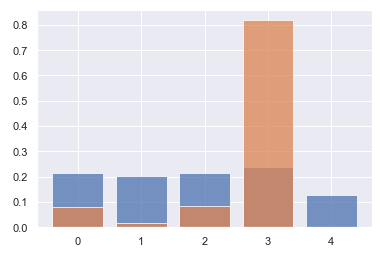
\includegraphics[width=0.5\textwidth]{entropy_discrete.PNG}\label{fig:entropy_discrete}}
  \hfill
  \subfloat[Continuous probability distribution $p(a|s)$]{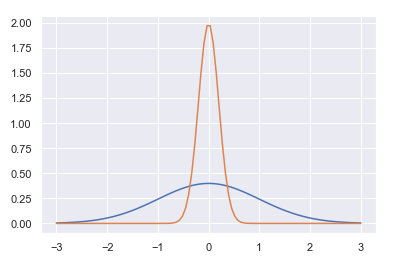
\includegraphics[width=0.5\textwidth]{entropy_cts.PNG}\label{fig:entropy_cts}}
  \caption{Orange shows low-entropy distributions. Blue shows high-entropy distributions.}
  \label{fig:entropy}
\end{figure}

\subsection{Terminology}

Based on my understanding of RL literature, `entropy' technique in RL normally refers to `entropy regularization'. `entropy regularization' technique includes but not limited to adding `entropy bonus' in objective function and using `maximum-entropy'. `entropy bonus' includes but not limited to `one-step (naive) entropy bonus' and `proper entropy bonus'. The term `entropy bonus' is usually a constant or a vector of real numbers. `one-step entropy bonus' only applies to the current state, while `maximum-entropy' optimizes over the long-term sum of entropy. There is also a technique to maximize over both long-term rewards and long-term entropy. This is referred to as maximum entropy reinforcement learning.



\subsection{Why use entropy in RL}

It is a common practice to use entropy regularization to ensure policy exploration in policy gradient methods \cite{odonoghue2017combining}.
An agent might be stuck in a local optimum or never finding the global optimum because of not exploring the behavior of other actions.
Entropy encourages exploration, avoiding the situations where agent might fall into a local optimum.
This is critical for tasks with sparse reward because the agent seldomly receives feedback for its action, and therefore might overestimate some reward received and repeat the actions that led to that reward. With improved exploration, the agent will be more robust to abnormal or rare events while developing a task.

Other benefits of using entropy includes augmenting RL objective \cite{brianEntropy2010}, encouraging longer episodes \cite{schulman2018equivalence}, fine-tuning policies and better adaptability to new environments \cite{haarnoja2017reinforcement}.



\subsection{How to use entropy in RL}

In information theory, entropy for a discrete random variable $x$ is defined as: 
\begin{equation}
\label{eqn:info_entropy}
H(X) = -\sum_{x\in X} P(x) logP(x)
\end{equation}
In RL, the formula becomes Equation \ref{eqn:rl_discrete_entropy} as we calculate the entropy of the policy $\pi(a|s_t)$ for discrete action space (replace sum with integral for continuous action space).
\begin{equation}
\label{eqn:rl_discrete_entropy}
H(\pi(\cdot|s_t)) = -\sum_{a\in \mathcal{A}} P(x) log P(x)
\end{equation}

It is typical to add an `entropy bonus' term to the loss function, which encourages the agent to take actions more unpredictably so as to counteract the tendency of falling into local optimum \cite{odonoghue2017combining}.
For example, in A3C \cite{mnih2016asynchronous}
\[
\nabla_{\theta'}log\pi (a_t | s_t; \theta')(R_t - V(s_t;\theta_v))+\beta\nabla_{\theta'}H(\pi(s_t;\theta'))
\]
where $H(\pi)$ is the entropy bonus term, and the hyperparameter $\beta$ controls the strength of the entropy regularization term. \cite{mnih2016asynchronous} found that adding the entropy of the policy $\pi$ to the objective function improved exploration by discouraging premature convergence to suboptimal deterministic policies.

For one more example, \cite{schulman2018equivalence} discussed naive and proper entropy bonuses for A2C (advantage actor critic; a well-tuned version of A3C). The entropy bonus term is added in following way:

naive / one-step entropy bonus:
\[
\nabla log \pi_\theta (a_t | s_t) \bigg( \sum_{d=0}^{n-1} \gamma^d r_{t+d} - V(s_t) \bigg) - \tau \nabla_\theta \underbrace{ D_{KL} [\pi_\theta || \bar{\pi} ] (s_t)}_\text{entropy bonus}
\]

proper entropy bonus:
\[
\nabla log \pi_\theta (a_t | s_t) \bigg( \sum_{d=0}^{n-1} \gamma^d (r_{t+d} - \tau \underbrace{ D_{KL}[\pi_\theta || \bar{\pi}](s_{t+d})}_\text{entropy bonus} ) - V(s_t) \bigg) - \tau \nabla_\theta \underbrace{ D_{KL} [\pi_\theta || \bar{\pi} ] (s_t) }_\text{entropy bonus}
\]

A side note for training: entropy should slowly and consistently decrease during a successful training process. If it decreases too quickly, the entropy coefficient hyperparameter should be increased.


\subsection{Further reading}

Application of entropy (regularization) in RL is a well-studied topic, some notable paper in this area:

\begin{itemize}
\item \cite{ahmed2019understanding} Understanding the impact of entropy on policy optimization
\item \cite{schulman2018equivalence} Equivalence Between Policy Gradients and Soft Q-Learning
\item \cite{haarnoja2017reinforcement} Reinforcement Learning with Deep Energy-Based Policies (soft (entropy-regularized) Q-learning)
\item \cite{nachum2017bridging} Bridging the Gap Between Value and Policy Based Reinforcement Learning (entropy bonus)
\item \cite{odonoghue2017combining} Combining policy gradient and q-learning (entropy bonus)
\item \cite{mnih2016asynchronous} Asynchronous Methods for Deep Reinforcement Learning (A3C)
\item \cite{brianEntropy2010} Modeling purposeful adaptive behavior with the principle of maximum causal entropy
\item \cite{Williams1992SimpleSG} Simple statistical gradient-following algorithms for connectionist reinforcement learning
\end{itemize}

Related topics include one-step entropy vs. maximum entropy, and entropy vs. KL-divergence as regularizer.

\section{Discounted Reward vs. Average Reward}

As disscussed in Chapter 10.3 and 10.3 of \cite{Sutton1998}, discounted reward and average reward can both apply to continuing problems; however, discounted reward is problematic with function approximation, and thus the average reward is needed to replace it.

In the average reward setting, the quality of a policy $\pi$ is defined as \textit{average reward}, denoted as $r(\pi)$:
\begin{align*}
r(\pi) & \doteq \lim_{h \to \infty} \frac{1}{h} \sum_{t=1}^{h} \E [R_t | S_0, A_{0:t-1}\sim \pi]\\
& = \lim_{t \to \infty} \E [R_t | S_0, A_{0:t-1}\sim \pi]\\
& = \sum_s \mu_\pi(s) \sum_a \pi(a|s) \sum_{s',r} p(s',r|s,a)r
\end{align*}
where the expectations are conditioned on the initial state, $S_0$, and on the subsequent actions, $A_0, A_1, \dots, A_{t-1}$, being taken according to $\pi$. The second and third equations hold if the steady-state distribution $\mu_\pi(s) \doteq \lim_{t\to\infty}P(S_t = s | A_{0:t-1}\sim\pi)$ exists and is independent of $S_0$, in other words, if the MDP is \textit{ergodic}\footnote{A random process $X(t)$ is ergodic if all of its statistics can be determined form a sample function of the process; that is, ensemble averages = corresponding time average. In plain terms, a system is ergodic if its long-term behavior behaves almost independently of initial conditions.}.
In an ergodic MDP, in the long run the expectation of being in a state depends only on the policy and the MDP transition probabilities.

In the average-reward setting, returns are defined in terms of differences between rewards and the average reward:
\[
G_t \doteq R_{t+1} - r(\pi) + R_{t+2} - r(\pi) + R_{t+3} - r(\pi) + \cdots
\]
which is known as the \textit{differential return}, and the corresponding value functions are known as \textit{differential} value functions.

The bellman equation in differential forms:
\begin{align*}
v_\pi(s) & = \sum_a \pi(a|s) \sum_{r,s'} p(s',r|s,a)[r-r(\pi)+v_\pi(s')]\\
q_\pi(s,a) & = \sum_{r,s'}p(s',r|s,a)[r-r(\pi)+\sum_{a'}\pi(a'|s')q_\pi(s',a')]\\
v_{\pi_*}(s) & = \max_a \sum_{r,s'} p(s',r|s,a)[r-\max_\pi r(\pi)+v_{\pi_*}(s')]\\
q_{\pi_*}(s,a) & = \sum_{r,s'}p(s',r|s,a)[r-\max_\pi r(\pi)+\max_{a'}q_*(s',a')]
\end{align*}
TD errors in differential forms:
\begin{align*}
\delta_t & \doteq R_{t+1} - \bar{R_t} + \hat{v}(S_{t+1}, w_t) - \hat{v}(S_t, w_t)\\
\delta_t & \doteq R_{t+1} - \bar{R_t} + \hat{q}(S_{t+1},A_{t+1},w_t) - \hat{q}(S_t, A_t, w_t)
\end{align*}
where $\bar{R_t}$ is an estimate at time $t$ of the average reward $r(\pi)$.

The continuing, discounted problem formulation is very useful in tabular cases, in which the returns from each state can be separately identified and averaged. However, it is questionable to use continuing discounted formulation in approximate cases.

Consider an infinite sequence of returns with no beginning or end, and no clearly identified states. The states might be represented only by feature vectors, which is difficult to distinguish the states from each other. There are only reward sequence (and actions) to work on. To achieve this, we average the rewards over a long interval. Discounting can be added, but the average of the discounted rewards would be proportional to the average reward. To see this, consider:
each time step is exactly the same as other in continuing settings. With discounting, every reward will appear exactly once in each position in some return. The $t$th reward $r_t$ is undiscounted in $(t-1)$th reward, discounted once in $(t-2)$ return and discounted 999 times in the $(t-1000)$th return. The weight on the $t$th reward is thus $1+\gamma + \gamma^2 + \cdots = \frac{1}{1-\gamma}$ \footnote{Mathematical proof is shown in page 254 on \cite{Sutton1998}.}.
Since all states are the same, the average of the returns will just be $\frac{r(\pi)}{1-\gamma}$.
The discount rate $\gamma$ thus has no effect on the continuous problem formulation.

\end{appendices}


%%%%%%%%%%%%%%%%%%%%%%%%%%%%%%%%%%%%%%%%%%%%%%%
% References
%%%%%%%%%%%%%%%%%%%%%%%%%%%%%%%%%%%%%%%%%%%%%%%

\newpage
\bibliography{references_RLAlgo}


\end{document}
















